
\documentclass[12pt]{article}

\usepackage[margin=2cm]{geometry}
\usepackage{graphicx}
\usepackage{caption}
\usepackage{indentfirst}
\usepackage[numbers]{natbib}
\usepackage{float}

\begin{document}
	\title{\textsc{Analysis of Pass Distribution Networks on Football Teams}}  
	\author{\begin{LARGE}Andr\'{e} Diegues\end{LARGE}}
    \date{\today}  
    \maketitle
    %\vfill
    \begin{center} 
    DCC/FCUP
    \end{center}
	\thispagestyle{empty}
	\clearpage
	\tableofcontents
	\pagebreak
  \section{Introduction}\label{sec: intro}

What can we say to describe what is or what is not a network? A network is a set of vertices or nodes, with connections between them, called edges. Systems that take the form of networks are designated by graphs and almost everything can be represented in this form.
Nowadays, networks fit to represent some of the most important things in the world, like social networks like \textit{Facebook} or \textit{Twitter}, biological networks such as neurological networks, information networks like the network of citations between academic
papers and, lastly, technological networks which are all networks that are implemented by the human kind in the world such as water networks, transportation networks and even communication networks~\cite{Newman}. 

In this article we're going to represent through networks the pass distribution of football teams in the high-level of the sport looking specifically to the best European competition, the \textit{UEFA Champions League}. We are hoping to find patterns in the networks that can reveal, for example, who is the most influential player of a team, how the absence of that player impacts the performance of his team and also if the team's strategy is the same with and without that player.

\section{Building the Networks}\label{sec: build}

In order to represent all the teams in the \textit{UEFA Champions League} we had to get the pass distribution of these teams. Fortunately all the data from the season 2012/2013 till the present season was available on the \textit{UEFA} official website at \linebreak\texttt{http://www.uefa.org/mediaservices/presskits/uefachampionsleague/} in the total pass distribution .pdf files. We can see Figure~\ref{fig:tpd}, in the following page, as an example of these files.

\begin{figure}[H]
	\centering
	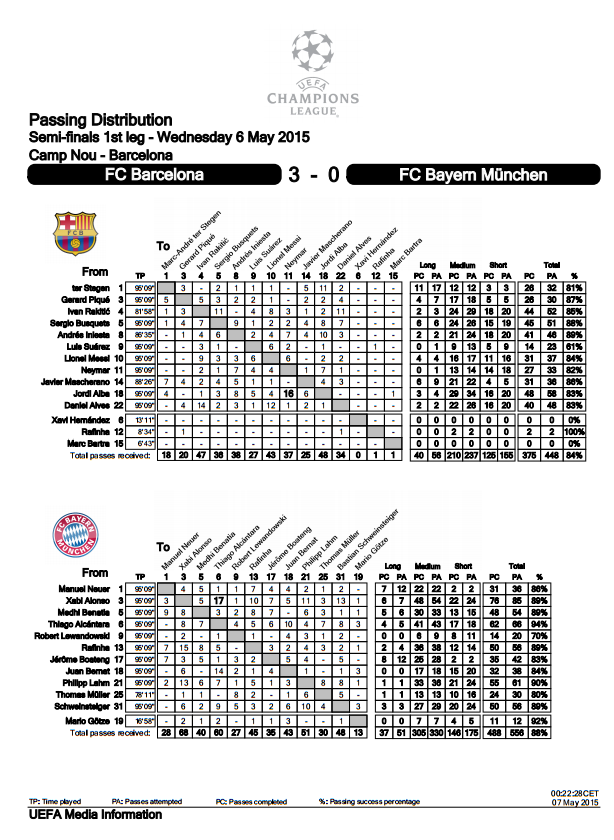
\includegraphics[scale=1]{tpd.png} 
	\caption{Example of a pass distribution file from the official \textit{UEFA} website}
	\label{fig:tpd}
	
\end{figure}

\subsection{Extracting the Data}\label{sec: extract}

Since the files are  .pdf files, the data isn't readable, in that case we implemented a JAVA program that would download the file and right after the download would convert the .pdf file into a .txt file. This program would automatically invoke, to all the pass distribution files available in the website, the \texttt{wget} command following from the \texttt{pdftotext -raw} command (the \texttt{raw} option guarantees the integrity of the data). 

\subsection{Collecting the Data into Data Structures}\label{sec: collect}

Like in the section \ref{sec: extract} we coded everything in JAVA. It is a object-oriented high level programming language with a very good API, a lot of documentation and community support, a very satisfying performance and exception handling that can provide flexibility when it comes to be creative. Creating a XML or SQL database wouldn't be necessary because we are not looking to be doing queries and JAVA has the particularity of free the allocated memory when the program terminates, the objective of this project is to study the pass distribution networks and all the queries can be easily done in JAVA if necessary. 

Analysing the converted .txt files, the data was all spread out and not organized at all. Due to this fact we decided to implement a JAVA program to parse the data in order to organize and, most importantly, to make it reliable and consistent. After that, the primary focus was to create data structures that could represent all the data found in one file.

Given some consideration we decided that we wanted each team to have a graph for each different season. In order to do that we implemented the following data structures:
\begin{enumerate}
	\item{Match}
	\begin{enumerate}
		\item{MatchScore}
		\item{MatchDate}
	\end{enumerate}
	\item{Player}
	\item{Team}
	\item{Season}
	\item{Pass}
\end{enumerate}

\subsection{Converting the Data into Networks}\label{sec: convert}

Now that the data is collected we need a tool to reproduce the data into networks. In the following section we'll introduce you to Gephi: An Open Source Software for Exploring and Manipulating Networks~\cite{bastian2009gephi}.


\subsubsection{Gephi}\label{sec: gephiSection}

Gephi is a powerful tool to visualize and analyse networks. It has a friendly and easy-to-use framework and the task of importing data is as easy as it can be. Anyone can build networks from spreadsheets or another file extensions, such as GraphML, GML, CSV and so on~\cite{gephi}. The Figure~\ref{fig:gephi} is an example of the capabilities of Gephi with respect to network visualization and analysis.

\begin{figure}[H]
	\centering
	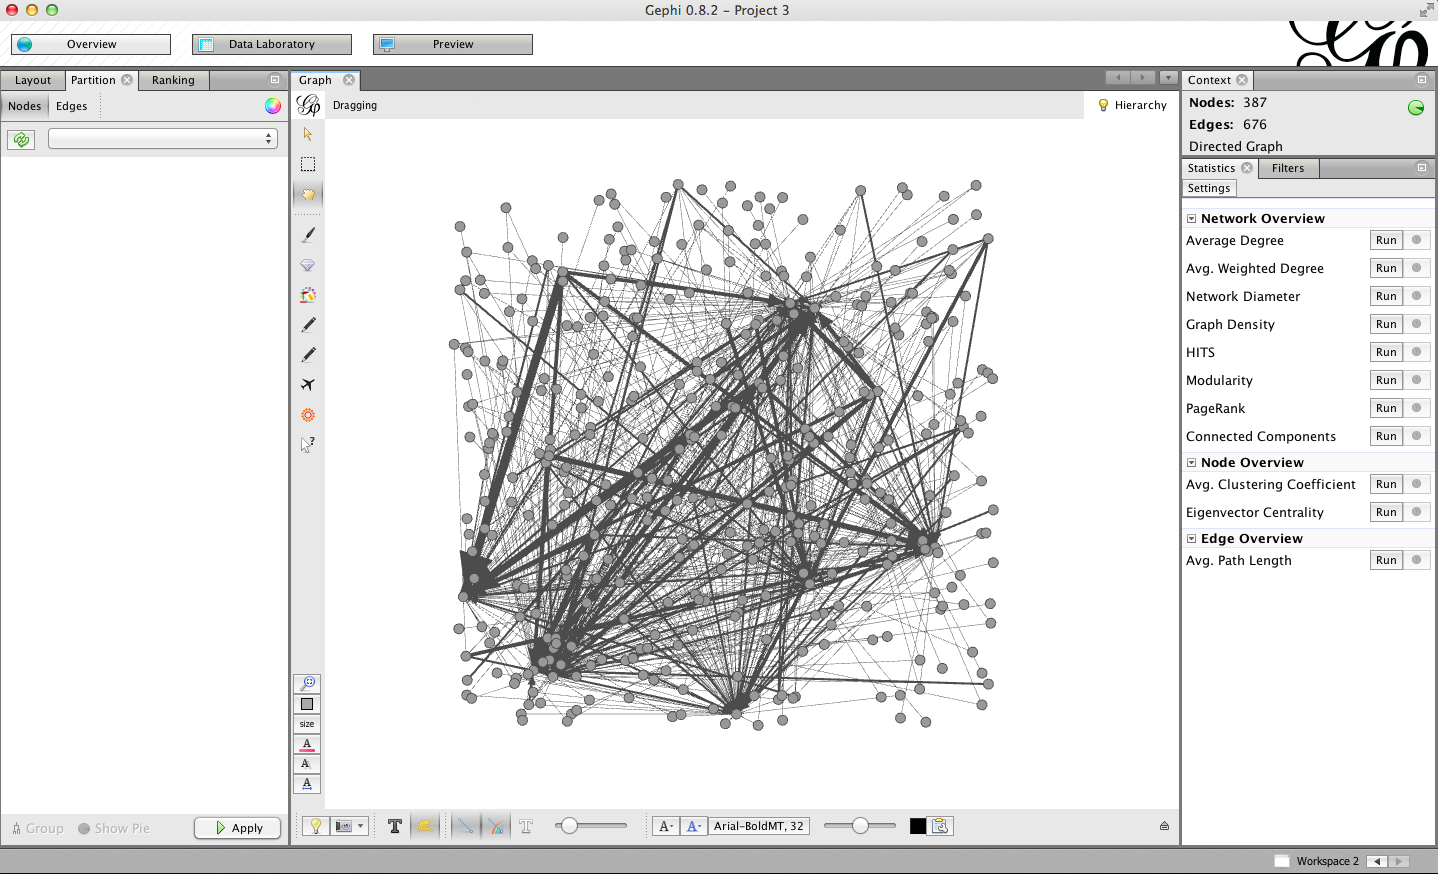
\includegraphics[scale=0.35]{gephi.png}
	\caption{Example of a network built in Gephi}
	\label{fig:gephi}
\end{figure}
\subsubsection{Parsing the Data}\label{sec: parser}

Since we're using Gephi to analyse our pass distribution networks, we needed to rearrange the data so it would be easier to import it to Gephi in the future. In this way, we would not waste time importing data to the platform. We've decided to parse the data in two formats:
\begin{enumerate}
	\item{Spreadsheet Notation}
	
The Spreadsheet Notation is very easy to read and understand the data. For this project, any spreadsheet presented like  Tables~1 and 2 can be easily imported into Gephi, we need only to specify which table represents the nodes and which table represents the edges and after that the network is built nice and easy. 
\begin{table}[H]\label{tab:Spreadsheet}
	\begin{minipage}{.5\linewidth}
	\centering
		\begin{tabular}{l|l}
			Id  & Name          \\
			\hline
			20  & Sergio Romero \\
			7   & Memphis Depay \\
			8   & Juan Mata     \\
			... & ...          
		\end{tabular}
	\caption{Example of nodes}
	\end{minipage}
	\begin{minipage}{.5\linewidth}
		\centering
		\begin{tabular}{l|l|l}
			Source & Target & Weight \\
			\hline
			20     & 10     & 3      \\
			20     & 11     & 1      \\
			20     & 12     & 8      \\
			...    & ...    & ...   		
		\end{tabular}
	\caption{Example of edges}
	\end{minipage}
\end{table}	
\pagebreak
	\item{GML Notation}
	
GML, Graph Modelling Language, consists of a hierarchical key-value lists and it features portability, simple syntax, extensibility and flexibility~\cite{gml}. As we can see in Figure \ref{fig:gml}, firstly we must declare the nodes of the network before the edges. By doing this, we guarantee that the hierarchical key-value lists condition is preserved, avoiding information to be lost in the process of  construction of the network.
\begin{figure}[H]
	\centering
	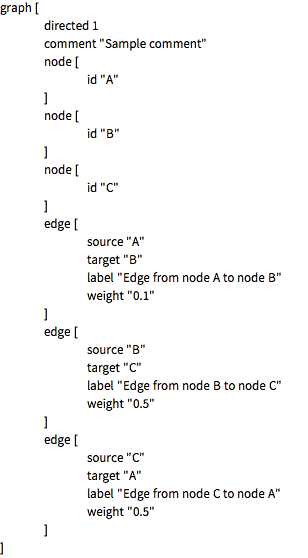
\includegraphics[scale=1]{gml.png}
	\caption{Example of a GML network}
	\label{fig:gml}
\end{figure}
\end{enumerate}
\newpage
\section{Results}\label{results}



\pagebreak
\bibliographystyle{plain}
\bibliography{report}

\end{document}